\documentclass[fleqn]{article} % For LaTeX2e
\usepackage{nips15submit_e,times}
\usepackage[hyperfootnotes=false]{hyperref}
\usepackage{url}
\usepackage{graphicx}
\usepackage[labelfont=bf]{caption}
\usepackage[outercaption]{sidecap} 
\usepackage{setspace}
\usepackage{amsmath}
\usepackage{amssymb}
\usepackage{footmisc}
\usepackage{enumitem}
\usepackage{xspace}

\makeatletter
\DeclareRobustCommand\onedot{\futurelet\@let@token\@onedot}
\def\@onedot{\ifx\@let@token.\else.\null\fi\xspace}
\def\eg{\emph{e.g}\onedot} \def\Eg{\emph{E.g}\onedot}
\def\ie{\emph{i.e}\onedot} \def\Ie{\emph{I.e}\onedot}
\def\cf{\emph{c.f}\onedot} \def\Cf{\emph{C.f}\onedot}
\def\etc{\emph{etc}\onedot} \def\vs{\emph{vs}\onedot}
\def\wrt{w.r.t\onedot} \def\Wrt{W.r.t\onedot} \def\dof{d.o.f\onedot}
\def\etal{\emph{et al}\onedot}
\makeatother

%\title{How Representations Affect Recognition Performances of Deep Networks?}
\title{What Makes a Deep Convolutional Representation Good for Visual Recognition?} % 

\author{
David S.~Hippocampus\\
Department of Computer Science\\
Cranberry-Lemon University\\
\texttt{hippo@cs.cranberry-lemon.edu} \\
}

\newcommand{\fix}{\marginpar{FIX}}
\newcommand{\new}{\marginpar{NEW}}

%\nipsfinalcopy % Uncomment for camera-ready version

\begin{document}

\maketitle

\begin{abstract}
Deep convolutional networks have been proven to be highly effective across a wide range of visual recognition tasks \cite{szegedy2014going, schroff2015facenet, donahue2014decaf}.
However, our understanding of how these networks work arguably remains limited.
Here, we examine two fundamental questions: first, why do deep networks outperform shallow networks, and second, among networks of the same depth, why do certain network architectures outperform the others.
We used face pair matching as a simplified recognition test-bed, and conducted a large-scale experiment in which random shallow and deep networks were generated and analyzed to measure properties of their resulting representations of visual inputs.
We describe a suite of measures of network selectivity, invariance, and representational quality that are able to account for up to 71\% of the variance in network performance, and we explore how these measures can yield insights into the factors that govern network performance.  
\end{abstract}

\begin{SCfigure}[1.5][h] % force here
\centering 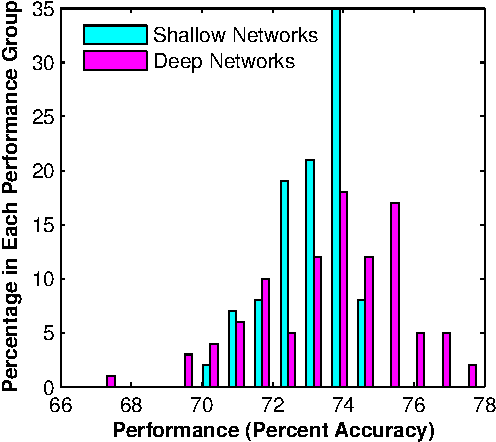
\includegraphics[width=0.40\textwidth]{Figs/perf.pdf} %\vspace{-1.5ex}
\caption{{\bf What makes a given deep network good?}
Among existing work, researchers mostly tried to produce one ``best'' network architecture (\ie a hyperparameter set, either through manual tuning or automated hyperparameter search), which is subsequently evaluated on a particular benchmark.
Nevertheless, it is not fully understood why in practice deep networks (\eg two or more levels) on average are better shallow networks (\eg one level), and why certain network architectures are better than the others, \eg when considering a larger population of networks \cite{cox2011beyond} and their distribution of performance (as shown here) on task like LFW-a face pair matching \cite{wolf2011effective} (see Sec.~\ref{sec:methods} for details of the experimental setup). \vspace{-0.5ex}}
\label{fig:perf}
\end{SCfigure}

\section{Introduction}

\newcommand{\expwhyface}{Nevertheless, the methods and most observations presented in this work are in general not limited to just face pair matching, and may be generalized onto other domains in visual recognition.}

In recent years, deep convolutional networks have come to dominate many benchmark challenges in computer vision, including datasets such as ImageNet \cite{russakovsky2014imagenet} and LFW \cite{LFWTech} year after year \cite{krizhevsky2012imagenet, sermanet2013overfeat, szegedy2014going, taigman2014deepface, sun2014deep, schroff2015facenet}.  However, in spite of this impressive performance, our understanding of these networks' properties arguably remains limited, since we cannot yet fully answer the question ``what makes a given deep network good?''
In this paper, we address two practical aspects of this important question: (1) why do deep networks perform better than shallow networks, and (2) among networks of the same depth, why do certain networks perform better than others (as illustrated in Fig.~\ref{fig:perf}).
More specifically, from the point of view that successful networks are forming better representations of visual inputs in which object categories are more separable, we want to identify the crucial properties that are required for forming (or learning) better representations. 
We adopted face pair matching (\ie identifying pairs of different pictures from the same person and rejecting those from different persons) as a benchmark task in our experiments, since previous investigations have shown that deep networks perform well in this domain \cite{taigman2014deepface}, and because face images can optionally be easily aligned and extracted from irreverent backgrounds, which can serve as a good source of visual stimuli for studying representations that fundamentally facilitates recognition.  The techniques presented here, however, are in no way specific to face recognition.

% for two main reasons: (1) representations of face recognition networks are far less studied than those of object recognition networks, and (2) face images can be easily aligned and extracted from irreverent backgrounds, which can serve as a better source of visual stimuli for studying representations that fundamentally facilitates recognition\footnote{\expwhyface}.

%\newcommand{\ivec}{\mathrm{vec}^{-1}}
\newcommand{\expstimdim}{For simplicity, a stimulus being 2-dimensional (\ie ${\bf{x}} \in \mathbb{R}^{\sqrt{N} \times \sqrt{N}}$) or vectorized (\ie ${\bf{x}} \in \mathbb{R}^N$) are used interchangeably.}

%first order, second order, flexibility
{\bf Existing work.} 
Given an artificial neural network $f$, the study of how $f$ represents a high dimensional stimulus\footnote{\expstimdim} ${\bf{x}} \in \mathbb{R}^N$ as a representation 
${\bf{r}}$ in existing work mainly focused on the first-order (\ie linear) characterization of $f$---the analysis of optimal stimuli, stimuli which lead to the strongest responses of given neurons.
For single-level convolutional networks using squared pooling, \ie $f_c({\bf{x}}) = \left\| {\bf{K}} \otimes {\bf{x}} \right\|_{F}$, the optimal stimulus was shown to be analytically approximable \cite{saxe2011random} using a Gabor-like filter, whether the convolution kernel $\bf{K}$ is structural or random.
For multi-level convolutional networks, the optimal stimuli of neurons from various depths were numerically approximated \cite{erhan2010understanding, ngiam2010tiled, le2012building, zeiler2014visualizing, simonyan2013deep} to qualitatively show neurons in deeper layers are tuned to more complex visual patterns.
The generalized concept of optimal stimulus when considering groups of neurons can also be adopted to study the representations by inverting them \cite{mahendran2014understanding}.

Beyond the first-order characterization, the analysis of invariance and selectivity properties of neurons (\eg changes in stimuli which given neurons are least and most sensitive to, how small or large the changes are, \etc) was also adopted in a few works.
This can be viewed as the second-order characterization of $f$, and parametric deformation in stimuli was the most commonly used setup.
For example, translation, rotation, scaling, \etc of the stimulus were used in \cite{goodfellow2009measuring, zeiler2014visualizing} to test the invariance and selectivity of neurons.
Similar deformations were also adopted in \cite{lenc2014understanding}, but extended to analyze more advanced properties (equivariance and equivalence) of groups of neurons.
More generalized setups that, \eg, utilize local quadratic information (\ie the Hessian) or ``global'' numerical searches in the stimulus space, are less explored in the context of artificial neural network studies. %even though they do exist, 
For quadratic networks, \ie $f_q\left({\bf{x}}\right) = \frac{1}{2}{\bf{x}}^{T}{\bf{Qx}}+{\bf{L}}^{T}{\bf{x}}+c$, through eigendecomposing the quadratic term $\bf{Q}$ (\ie the Hessian), local invariance and selectivity directions can be analytically derived \cite{berkes2006analysis}, which correspond to eigenvectors of the least and most negative eigenvalues.
This method also can be generalized onto multi-layer convolutional networks by numerically estimating the Hessian \cite{ngiam2010tiled}.
For multi-layer networks, characterization of the ``global'' invariance of single neurons can also be achieved by numerically searching for non-local (\ie farther to the optimal stimuli) solutions \cite{erhan2010understanding}.

While it is fully justifiable to qualitatively characterize and verify the effectiveness of representations in individual well-performing deep networks to be deployed in real applications, we however argue that this approach may not either teach us much about what really makes them good, and how to further improve them when even bigger training datasets are not easily available.
Since theoretical tools capable of fully harnessing these highly nonlinear networks still await discovery, we took a different route by studying a large population of networks and using statistical tools to help us sort out the crucial properties of better representations, through directly comparing representations from the shallow \vs deep networks, and the good \vs bad networks.

%{\bf Contributions of this work.} Comparatively, the characterization of representations in this work is designed to be general and unbiased such that both first- and second-order methods can be supported for single neurons or groups of neurons, without assuming any \emph{de facto} property in the solutions (\eg parametric deformations as used for studying invariance in previous works).
%Additionally, with the strong statistical significance of results obtained from the large-scale experiments on 100 shallow and 100 deep networks, totally 6,400 artificial neurons, we argue that our observations toward answering the differences between (shallow \vs deep) and among (deep) representations are highly evident and comprehensive, which cab be summarized as ***

%\section{Representation Characterization}
\section{Methods}
\label{sec:methods}

\begin{SCfigure}[1.5][t]
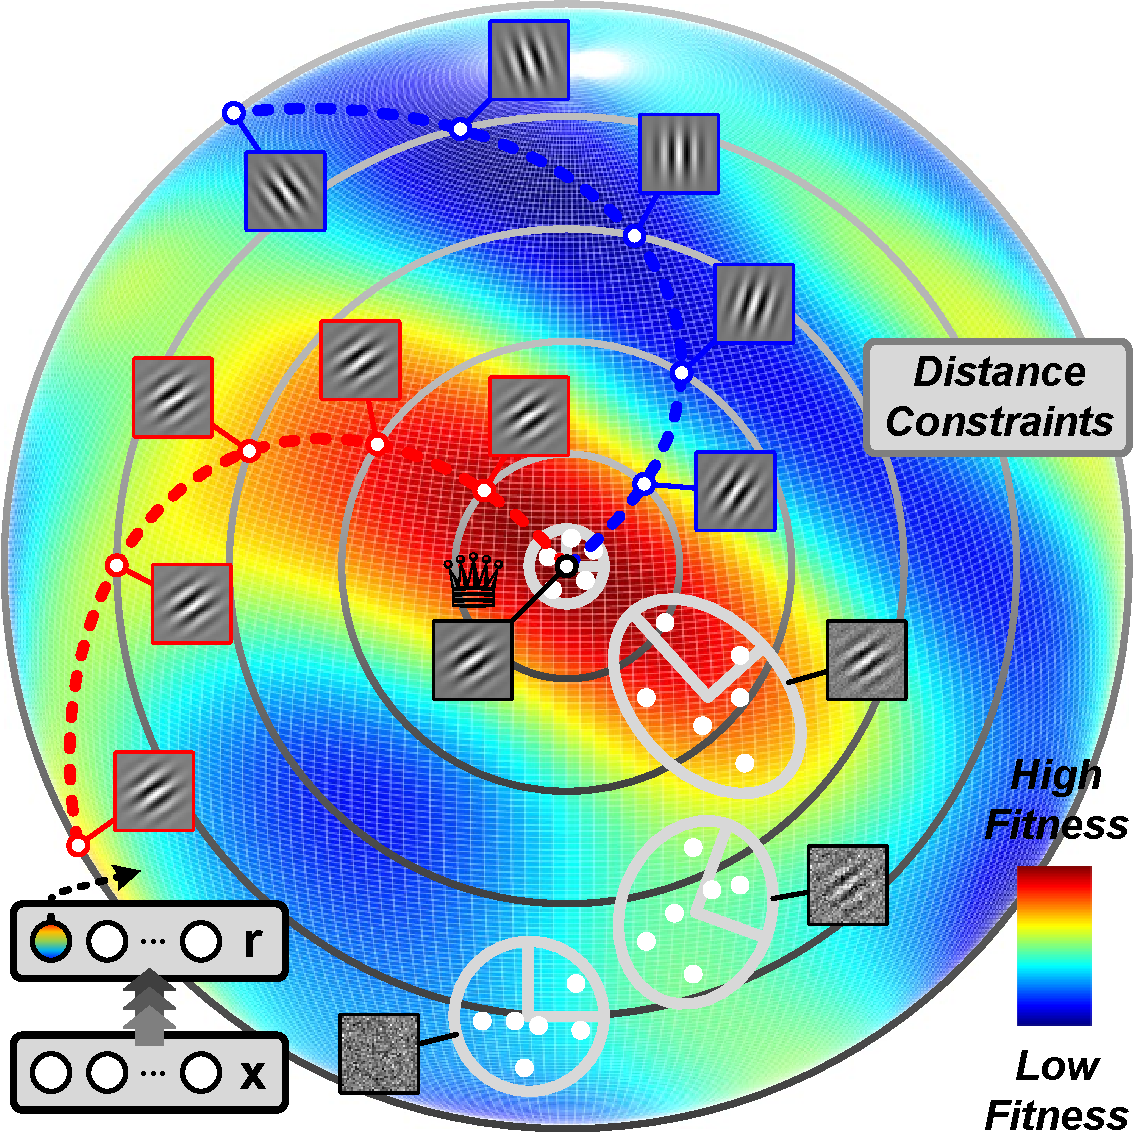
\includegraphics[width=0.40\textwidth, clip]{Figs/methods.pdf}
\caption{{\bf Outline of representation characterization.}
On the spherical (\ie constant energy) constraint of the $N$-dimensional stimulus space, the first-order property, \ie optimal stimulus $\hat{\bf{x}}$, of a representation $\bf{r}$ is first iteratively searched \cite{hansen2001completely} (as the evolution of gray eclipses) and analyzed.
Then, the second-order properties, \ie invariance path $\lbrace \bf{x}^{+}_{\delta} \rbrace$ and selectivity path $\lbrace \bf{x}^{-}_{\delta} \rbrace$ (as dashed red and blue curves) at distances $0.1\pi$ to $0.5\pi$ away from the optimal stimulus, are both searched and analyzed too.
In this example, the scalar representation (\ie response) of the given neuron is optimally tuned to the $45^{\circ}$ Gabor filter and invariant to phase changes, but selective to orientation changes.
\vspace{1.0ex}}
\label{fig:methods}
\end{SCfigure}

%representational property 

%similar to previous work,
%However, unlike most previous work
%These methods can also characterize both scalar and vector representations, in which the ``fitnesses'' to be optimized correspond to Eq.~\ref{eq:O1}, \ref{eq:I1}, \ref{eq:S1} and Eq.~\ref{eq:O2}, \ref{eq:I2}, \ref{eq:S2}, respectively.
% (linear) (quadratic-like) (\ie eigenvectors of the largest and smallest eigenvalues)

To study the representations inside an artificial neural network, methods adopted in this work include: (1) first-order characterization, or search and analysis of optimal stimuli, and (2) second-order characterization, or search and analysis of invariance and selectivity paths, which are generalized and improved from previous work.
Throughout the paper, $\bf{r}$ is defined as a scalar representation (\ie ${\bf{r}} = f_s\left({\bf{x}}\right) \in \mathbb{R}$) when considering single neurons and a vector representation (\ie ${\bf{r}} = f_v\left({\bf{x}}\right) \in \mathbb{R}^C$) when considering groups of neurons (with group size $C$).
The search (\ie numerical optimization) phases are defined via the following equations, and the analyses of search results using representation measures will be covered in Sec.~\ref{sec:results1} and \ref{sec:results2}. 
We denote the following functions being optimized as \emph{fitness functions} and their values as \emph{fitnesses}.

\setlength{\mathindent}{1.0ex}
\begin{minipage}[c]{0.33\textwidth}
\begin{align}
\hat{\bf{x}} &= \underset{\bf{x}} {\arg\max} \ f_s(\bf{x}) \label{eq:O1} \\
&= \underset{\bf{x}}{\arg\max} \ e^{-\left\|f_v({\bf{x}})-f_v(\tilde{\bf{x}})\right\|} \label{eq:O2}
\end{align}
\end{minipage}
\begin{minipage}[c]{0.33\textwidth}
\begin{align}
\bf{x}^{+}_{\delta} &= \underset{\bf{x}_{\delta}}{\arg\max} \ f_s(\bf{x}_{\delta}) \label{eq:I1} \\
&= \underset{\bf{x}_{\delta}}{\arg\max} \ e^{-\left\|f_v({\bf{x}}_{\delta})-f_v(\hat{\bf{x}})\right\|} \label{eq:I2}
\end{align}
\end{minipage}
\begin{minipage}[c]{0.33\textwidth}
\begin{align}
\bf{x}^{-}_{\delta} &= \underset{\bf{x}_{\delta}}{\arg\min} \ f_s(\bf{x}_{\delta}) \label{eq:S1} \\
&= \underset{\bf{x}_{\delta}}{\arg\min} \ e^{-\left\|f_v({\bf{x}}_{\delta})-f_v(\hat{\bf{x}})\right\|} \label{eq:S2}
\end{align}
\end{minipage}

\newcommand{\expconst}{We restrict the space of stimuli considered with a constant energy constraint $\left\| \bf{x} \right\| = E$, where $E$ in all mathematical derivations is set to $1$ for simplicity, but in our experiments, set to the average energy of task-related images. This avoids degenerate solutions that simply maximize stimulus contrasts.}
%While no specific knowledge of the network itself is assumed

The optimal stimulus of a scalar representation (\ie a single neuron) can be defined as Eq.~\ref{eq:O1} subject to $\left\| \bf{x} \right\| = 1$\footnote{\expconst}.
When considering a vector representation (using Eq.~\ref{eq:O2}), it is equivalent to optimizing the response of an ``auxiliary neuron'' tuned to a certain reference stimulus $\tilde{\bf{x}}$.
With respect to the optimal stimulus $\hat{\bf{x}}$, the invariant and selective stimuli can be defined using Eq.~\ref{eq:I1} and \ref{eq:S1} respectively, where $0 < \delta \le \frac{\pi}{2}$, subject to $\left\| \bf{x}_{\delta} \right\| = 1$ and $\langle {\bf{x}}_{\delta} , \hat{{\bf{x}}} \rangle = \cos\left(\delta\right)$. 
The distance constraint, while being simple and linear, enforces the exploration of the landscape, which is one of the main improvements too compared to \cite{erhan2010understanding}.
The invariance path $\left\lbrace \bf{x}^{+}_{\delta} \right\rbrace$ and selectivity path $\left\lbrace \bf{x}^{-}_{\delta} \right\rbrace$ are then derived through multiple runs of maximization and minimization on discretized $\delta \in \left\lbrace 0.1\pi, 0.2\pi, 0.3\pi, 0.4\pi, 0.5\pi\right\rbrace$ as the distance constraints shown in Fig.~\ref{fig:methods}, where each run is initialized with the result from the previous run (and the $0.1\pi$ run directly with optimal stimulus $\hat{\bf{x}}$) to increase the path continuity and searching speed.
This can also be performed with respect to certain reference stimulus $\tilde{\bf{x}}$, especially for vector representations (using Eq.~\ref{eq:I2} and \ref{eq:S2}), where the invariance and selectivity of the auxiliary neuron are equivalently characterized again.

\newcommand{\expsettings}{
\Ie 32 channels of filters in the top level's convolution layers, a simple setting yielding reasonable performances.
Following the terminology in recent papers, shallow and deep neurons corresponded to \texttt{pool1} and \texttt{pool2} layers respectively.
Stimulus dimensionalities of the shallow and deep neurons {were} $N=121$ and $441$ (\ie spatially overlapping $11\times11$ and $21\times21$ receptive fields). % respectively
Other minor changes included: nonlinear activations all simplified to \emph{ReLU} \cite{krizhevsky2012imagenet} mode and normalizations all in subtractive mode.
Overall, the architectures were more similar to those in \cite{simonyan2014very}, except pooling operations can be \emph{average}, \emph{squared}, or \emph{max-like} in our case.
}

% \cite{fukushima1980neocognitron, lecun1998gradient, riesenhuber1999hierarchical, krizhevsky2012imagenet}
\newcommand{\expperf}{10-fold cross validation accuracies using the LFW view 2 splits (\cite{LFWTech}, totally 6,000 face pairs) are reported.
Although it is highly desirable to characterize representations from the state-of-the-art face pair matching networks \cite{taigman2014deepface, sun2014deep, schroff2015facenet}, neither those trained networks nor their datasets are publicly available.
Nonetheless, under the hard protocol adopted here (\ie image-restricted, no outside data, data augmentation, or multiple-crop evaluation), the (well-performing) random networks remain competitive against trained networks and do provide good representations in terms of accuracies attained.
} 
%State-of-the-art networks trained on massive private datasets \cite{taigman2014deepface, sun2014deep, schroff2015facenet} do have significantly higher accuracies. %absolute
%However, under the hard protocol adopted here (\ie image-restricted, no outside data), this model remains competitive among neural network-based algorithms.
%accuracy of identifying pairs of different pictures from the same person and rejecting those from different persons

{\bf Experimental setup.}
To enable the rapid probing of a large number of candidate networks, we used simplified random (untrained) deep convolutional neural networks \cite{cox2011beyond, sthor} in our experiments.
As with other deep networks, these networks consist of the standard cascade of convolution, nonlinear activation, pooling layers, \etc (which together define a single ``level'' in this work), however, the convolution kernel weights are randomly assigned rather than trained.
Though not fully matching the performances of deep networks trained on massive quantities of data, such models nonetheless surprisingly effective in regimes where limited training data is available \cite{cox2011beyond}. %\eg the LFW-a setting we used \cite{krizhevsky2012imagenet} \cite{pinto2009high, cox2011beyond, viglarge}.
Most importantly, since the networks themselves do not require training---except for a simple linear classifier at the final stage of the network---a large number of networks with diverse architectures and hyperparameters can be rapidly generated and compared, which is particularly useful in this study where relative, instead of absolute task performances, are of primary interest.
In the experiments, 100 shallow (\ie one-level) networks and 100 deep (\ie two-level) networks {were} randomly generated (except all with 32 top-layer neurons\footnote{\expsettings}) and tested to see how their representations differ with the networks' depths and affect the networks' performances on face pair matching against the LFW-a dataset \cite{wolf2011effective} as shown in Fig.~\ref{fig:perf}\footnote{\expperf}.

\section{Results: Shallow \vs Deep Representations}
\label{sec:results1}

\begin{figure}[t]
\centering 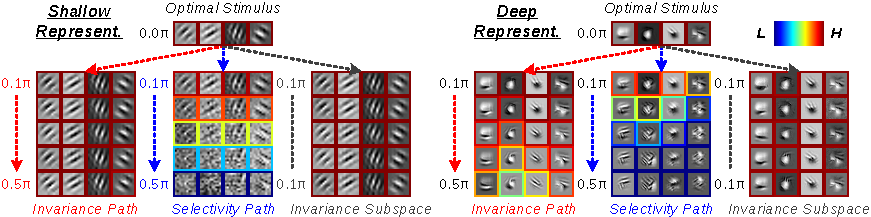
\includegraphics[width=\textwidth]{Figs/s_vs_d_repr.pdf} 
\caption{{\bf Visualization of shallow and deep representations.} %scalar
Representations of 4 neurons randomly selected (out of all 32 neurons) from the best performing shallow and best performing deep networks are shown in the left and right panels respectively. 
The optimal stimuli, invariance paths, selectivity paths, and invariance subspaces (sampled using invariant stimuli $0.1\pi$ away from the optimal stimuli; 5 out of 20 results randomly selected) of the 4 shallow and deep neurons are ordered and shown accordingly, where color of the boarder of an image indicates the fitness of the representation (\ie response of the neuron) elicited by the image.
See supplementary material for more examples.
Comparatively, \emph{deep neurons show more complex and diverse representational properties} than shallow neurons do.
} % do visually
\label{fig:allrep1}
\end{figure}

{\bf Optimal stimulus spectral complexity.}
Figure \ref{fig:allrep1} demonstrates examples of the optimal stimuli of neurons from the best performing (\ie best LFW-a accuracy) shallow and the best performing deep network.
The optimal stimuli of deep neurons are visually much more complex (\ie consisting of more textural components) than those of shallow neurons (which are more uni-textured or Gabor-like).
To quantify such differences, the spectral complexity measure defined as the $L^{1}$ norm of the 2-dimensional Fourier power spectrum of optimal stimulus, \ie $\left\| \mathcal{F}(\hat{\bf{x}}) \right\|_{1}$, is adopted, where a higher value suggests higher non-sparsity (\ie more spectral components required to represent the visual stimuli).

% trajectories -> SI

\begin{figure}[t]
\centering 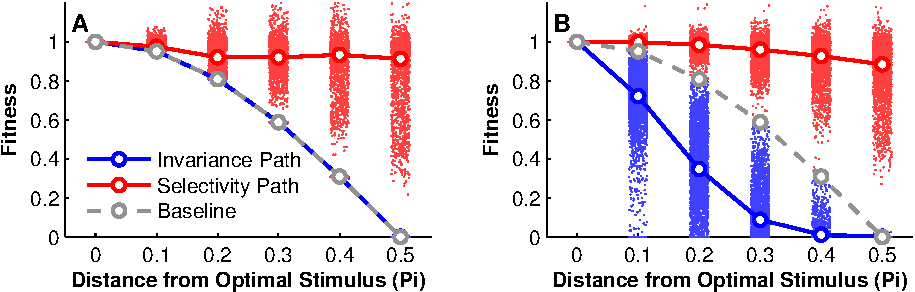
\includegraphics[width=0.80\textwidth]{Figs/fda.pdf} 
\caption{{\bf Fitness-distance analyses of shallow and deep representations.} %scalar
Fitnesses of invariance (red dots, \ie $\left\lbrace f_s(\bf{x}^{+}_{\delta}) \right\rbrace$) and selectivity paths (blue dots, \ie $\left\lbrace f_s(\bf{x}^{-}_{\delta}) \right\rbrace$) of all 3,200 shallow (panel A) and 3,200 deep neurons (panel B) are shown for comparison\protect\footnotemark.
Although both types of neurons show invariance, shallow neurons do not posses selectivity, since their selectivity paths overlap with the zero-selectivity baseline (see text for definition), \ie \emph{only deep neurons are selective}.
}
\label{fig:fda}
\end{figure}

\footnotetext{A small fraction of invariance paths actually have fitnesses higher than the optimal stimuli's, due to the non-convexity of these networks, which however does not lead to noticeable differences in the results in Fig.~\ref{fig:pair}.}

\newcommand{\defbaseline}{Given a single inner-product neuron $f_n({\bf{x}}) = {\bf{w}}^{T}{\bf{x}}$ and $\left\| \bf{x} \right\| = 1$, we have $\hat{\bf{x}} = \bf{w}$ and thus the invariance (and selectivity) curve $f_n({\bf{x}}_{\delta}) = \langle \hat{\bf{x}} ,{\bf{x}}_{\delta} \rangle = \cos(\delta)$ by definition.}

{\bf Invariance and selectivity path potential.}
Figure \ref{fig:allrep1} also illustrates the invariance and selectivity paths of the same sets of shallow and deep neurons as aforementioned.
While invariance paths are mostly phase changes and selectivity paths are leading toward meaningless noises (all at the same falloff rate) in shallow neurons, both types of paths consist of sophisticated shape deformations in deep neurons.
Interestingly, although most shallow neurons are also selective to manually rotated optimal stimuli (\ie Gabor filters of different orientations) as well, their fitnesses still do not drop faster then the nonparametric numerical solutions as presented in Fig.~\ref{eq:I1}.
As further demonstrated in the fitness-distance diagrams \cite{jones1995fitness} (Fig.~\ref{fig:fda}), on average, although shallow neurons have good invariance (\ie red curve stays high), they do not have any selectivity (\ie blue curve drops slow), while deep neurons show both good invariance and selectivity (\ie red curve stays high and blue curve drops fast).
For scalar representations, we can define the invariance (and selectivity, similarly) path potential as the area sandwiched between the invariance curve and the baseline curve (\ie the invariance curves of a single inner-product neuron\footnote{\defbaseline}---the ``baseline'' of all types of neural networks) on the diagram, \ie $\int_{0}^{0.5\pi} \left| \cos^{-1}(f_s(\bf{x}^{+}_{\delta} )) - \delta \right| \mathrm{d}\delta$ (in the $\cos^{-1}$ domain for equalizing both types of path potentials), which measures how invariant (and selective) a neuron is compared to the baseline. %/ {\frac{\pi}{2}}

%(zero-invariance/-selectivity)
%In fact, this intriguing difference generalizes across all shallow \vs deep neurons experimented in this work.

\newcommand{\expnoslsc}{Selectivity subspace capacity, on the other hand, is not a fair measure and thus not included, since shallow neurons do not even have selectivity close to deep neurons', and in a sense have more diverse ``most selective'' paths---noises.}

{\bf Invariance subspace capacity.}
To further characterize the properties of invariance, multiple runs of invariance path searches {were} performed, and the results are also visualized in Fig.~\ref{fig:allrep1}.
The constitution of the ``invariance plateau'' (\ie the central high fitness region in Fig.~\ref{fig:methods}) of deep neurons is much more diverse than that of shallow neurons.
In addition to the invariance path potential, which is designed to characterize the ``best invariance path'' even when only one of such exists, we further adopted the invariance subspace capacity measure\footnote{\expnoslsc} to estimates the ``dimensionality'' (\ie how diverse different paths can be) of the linear subspace formed by multiple path search results using the nuclear norm of the concatenation of $n$ results $\left\|\left[{\bf{x}}_{\delta,1},\dots,{\bf{x}}_{\delta,n}\right]\right\|_{*}$ with $n=20$ and $\delta=0.1\pi$.

%(\ie dimensionality, or subspace capacity) 

\begin{SCfigure}[1.5][t]
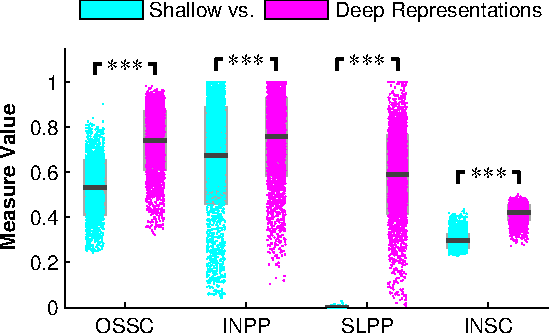
\includegraphics[width=0.40\textwidth]{Figs/s_vs_d.pdf} %\vspace{2.5ex}
%\begin{minipage}{0.40\textwidth}
%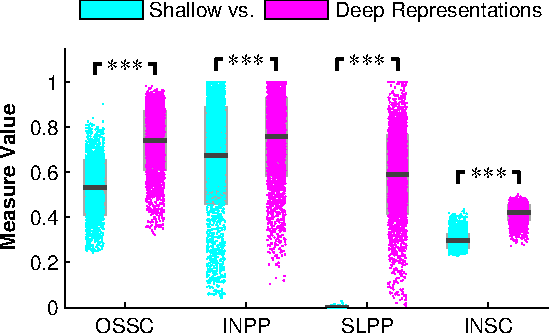
\includegraphics[width=\linewidth]{Figs/s_vs_d.pdf} %\vspace{-1.0ex}
%\scalebox{0.59}{\textsf{\emph{OSSC: Optimal Stimulus Spectral Complexity, INPP: INvariance Path Potential, SLPP: SeLectivity Path Potential, INSC: INvariance Subspace Capacity.}}}
%\end{minipage} 
\caption{{\bf Representation measures \vs depth of networks.} %scalar
Bhattacharyya distances and their significance levels\protect\footnotemark~between the 4 shallow and deep measures from left to right are $0.39^{\ast\ast\ast}$, $0.07^{\ast\ast\ast}$, $6.42^{\ast\ast\ast}$ and $1.27^{\ast\ast\ast}$ respectively, which suggest \emph{deep representations are quantitatively and significantly better than shallow representations}. \vspace{2.0ex} \\
\tiny{\textsf{\emph{OSSC: Optimal Stimulus Spectral Complexity, INPP: INvariance Path Potential, SLPP: SeLectivity Path Potential, INSC: INvariance Subspace Capacity.}}}
\vspace{1.5ex}}
\label{fig:pair}
\end{SCfigure}

\footnotetext{Significance levels *, **, and *** indicate $p<0.05$, $p<0.01$, and $p<0.001$, respectively, where all $p$-values {are} calculated using permutation tests (see supplementary material for algorithmic details). \label{fnote:defstars}}

{\bf Overall comparison.}
Comparisons of spectral complexities, invariance/selectivity path potentials, and invariance subspace capacities of all shallow and deep neurons (\ie scalar representations) are summarized in Fig.~\ref{fig:pair}.
These measures more precisely quantify the significant differences between shallow and deep representations, in comparison to the qualitative visualizations \cite{erhan2010understanding, ngiam2010tiled, zeiler2014visualizing} and separability/classifiability analysis \cite{donahue2014decaf, zeiler2014visualizing} adopted in previous studies.
For example, subtle differences of visual features have better chances being distinguished when the ``gap'' between the invariance and selectivity curves (\ie the dynamic range of neuronal responses, or amplification ratio of differences) is larger.
The highly structural representations of neurons from deep networks using purely random convolution kernels observed in the experiments also explain why such ``random'' deep networks can still have good performances, on top of the theoretical analysis for the one-level shallow networks \cite{saxe2011random}. %ADD MORE?

%The increase of complexities in deeper neurons' preferred/optimal stimuli also agrees with neurobiological findings in higher visual cortical areas (\eg V2 and V4 \cite{hegde2000selectivity, pasupathy2001shape}). 

\section{Results: Good \vs Bad Representations}
\label{sec:results2}

\begin{figure}[t]
\centering 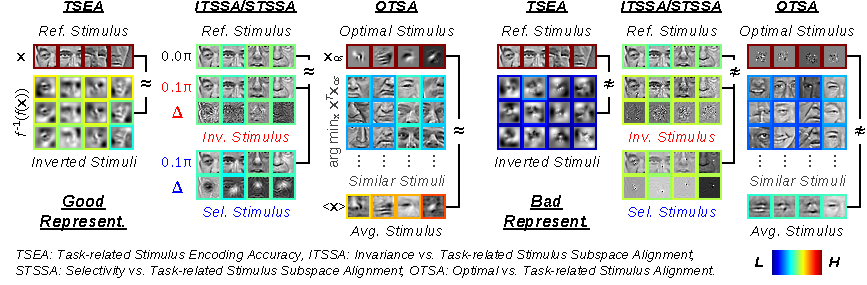
\includegraphics[width=\textwidth, trim=1.4ex 0.5ex 0 0, clip]{Figs/g_vs_b_repr.pdf} 
\caption{{\bf Visualization of good and bad representations.}
Good and bad examples from 3 types of the representation measures among all deep networks are shown in the left and right panels respectively, where color of the boarder of an image indicates its value of the corresponding representation measure (see text for definitions). %representation characterizations
(1) \Wrt the TSEA measure, good representations can be inverted with much stronger similarities to the original reference stimuli.
(2) \Wrt the ITSSA/STSSA measures, the ``intrinsic'' invariant and selective directions ($\Delta$'s, differences between the reference and invariant/selective stimuli $0.1\pi$ away) of good representations are much more natural (like structural deformations, lighting changes, \etc), and the invariant and selective stimuli align better against the eigenface subspace, whereas those of bad representations are highly noisy and align poorly against the eigenface subspace.
(3) \Wrt the OTSA measure, the optimal stimuli of good representations are comparatively more correlated to face images, especially to the linear averages of the most similar (top 100) face images, whereas those of bad representations do not.
Comparing these measures against the performances of deep networks (see Fig.~\ref{fig:corr}) shows strong correlations, which implies taht these first- and second-order properties of good representations must ``align with'' the distribution of task-related stimuli, even if the networks were not explicitly trained to have this property.
}
\label{fig:allrep2}
\end{figure}

{\bf Task-related stimulus encoding accuracy.}
To understand the meaning of a vector representation ${\bf{r}}$ formed by a deep network $f$, the inverse function $f^{-1}\left( \bf{r} \right)$ {was} numerically approximated (using Eq.~\ref{eq:O2}) to reveal what kind of stimulus can drive the deep network to give output $\bf{r}$.
Instead of inverting a randomly generated $\bf{r}$, which may not have feasible or interpretable solutions, we {used} $\bf{r}$ from known reference stimuli $\lbrace\tilde{\bf{x}}\rbrace$ (specifically, task-related stimulus, \ie randomly sampled face patches from the LFW-a dataset \cite{wolf2011effective}) to quantify the encoding accuracy and its relationship to performance.
Figure \ref{fig:allrep2} shows the reference stimuli and good \vs bad examples of encoding accuracies, where the average of structural similarities (SSIM) \cite{wang2004image} between the task-related reference stimulus $\tilde{\bf{x}}$ and $n$ inverted stimuli from multiple random initializations, \ie $\frac{1}{n}\sum_{i=1}^{n} \mathrm{SSIM}\left(\tilde{\bf{x}} , \hat{{\bf{x}}}_i \right)$ with $n=10$, is measured to estimate how accurate (\ie non-confounding) a representation is encoded.
This can also be interpreted as the first-oder alignment between the ``encoding landscape'' (\ie fitness landscape of the auxiliary neuron) and the task-related stimuli.
Our analysis predicts that strong encoding accuracies should also be observed in those even deeper and more powerful state-of-the-art networks. 
Interestingly, this in fact has been independently verified in recent studies \cite{mahendran2014understanding, long2014convnets, razavian2014persistent}, which also employed such kind of ``invertibility'' to study the representations. % of individual well-performing deep networks.
In addition, even though the deep convolutional representations used here are not formulated to be invertible (as opposed to, \eg, autoencoders), our results further suggest that this property can actually be \emph{required} for a deep network to perform well.

%SSIM measured using default settings of the standard implementation \cite{wang2004image} while different settings also yield similar correlations; other similarity measures like SNR, PSNR, and inner-product distance yield similar correlations as well

{\bf Invariance and selectivity \vs task-related stimulus subspace alignment.} 
It is widely known that invariance and selectivity are essential for biological vision \cite{desimone1991face, ito1995size}; however, how these properties directly affect the recognition performances of artificial neural networks remains unclear.
To address this question, starting from randomly sampled reference stimuli, invariance and selectivity path searches {were} performed at $\delta = 0.1\pi$ using Eq.~\ref{eq:I2} and \ref{eq:S2} for vector representations. 
Figure \ref{fig:allrep2} demonstrates examples of good and bad alignments between the subspaces formed by the invariance/selectivity paths and the task-related stimuli (\ie how likely the invariance and selectivity can benefit recognition), which are defined as the sparsity of $n$ paths projected onto the task-related stimuli's principal component (or here, eigenface) vector space $\bf{V}$, \ie $\frac{1}{n}\sum_{i=1}^{n} \left\| {\bf{Vx}}_{\delta,i} \right\|_{1}$ with $n=20$ and $\delta=0.1\pi$.
Compared to some previous work, our method does not assume that any kind of parametric deformation is important and thus should be studied.
Instead, the ``intrinsic'' invariant and selective directions of representations are directly searched and compared against the distribution of the task-related stimuli, which is relatively bias-free.
Surprisingly, highly natural invariance/selectivity are again observed in well-performing networks even given their nature of randomness.

%preferred
%$\left\lbrace {\bf{x}}^{t} \right\rbrace$
%quiroga2005invariant
%It can be observed that good alignments (\ie sparser representations in the principle component vector spaces) correspond to highly structural deformations or lighting changes, which are known to be important factors in visual recognition, while bad alignments correspond to mostly meaningless noises.

{\bf Optimal \vs task-related stimulus alignment.}
To understand how the optimal stimuli of individual neurons may affect a deep network's performance, we {measured} how well the optimal stimuli linearly aligns with the task-related stimuli, and how the alignment correlates with a network's performance.
Specifically, 10,000 face patches in total {were} randomly sampled from the LFW-a dataset and compared against the optimal stimuli of deep neurons.
Figure \ref{fig:allrep2} shows examples of good and bad alignments between the optimal stimuli and task-related stimuli, where the alignment measure is defined as the mean of the inner-product distances between an optimal stimulus and its $n$ nearest task-related stimuli $\left\lbrace {\bf{x}}^{t} \right\rbrace$, \ie $\frac{1}{n}\sum_{i=1}^{n} \langle {\bf{x}}^{t}_{i} , \hat{{\bf{x}}} \rangle$ with $n=100$, to estimate how well an optimal stimulus can linearly represent the task-related stimuli (or intuitively how responsive the corresponding neuron might be under the task).
Intriguingly, though none of the optimal stimuli is apparently similar to any of the task-related stimuli, when alternatively compared against the averages of the better aligned task-related stimuli (top 1\%), the similarities (in good representations) and dissimilarities (in bad representations) become apparent.
While it is unclear how to ``optimally place'' an optimal stimulus (or shape the entire landscape) in a high dimensional stimulus space under visual recognition tasks, based on our observations, we hypothesize that it should be closely surrounded by multiple visually similar task-related stimuli, such that the neuron is more likely to represent those similar stimuli (and only those stimuli) with similar values.
This observation may also explain why optimal stimuli often resemble the averages \cite{le2012building} or combinations \cite{simonyan2013deep} of multiple visual objects.

% (which in low dimensional cases are theoretically validated)
%Such kind of ``linearities'' around task-related images out of the well-performing highly-nonlinear networks were observed in previous studies \cite{le2012building, simonyan2013deep} too, where optimal stimuli also resembled averages or combinations of visual objects.
%much neuronal response might be elicited
%Specifically, 10,000 image patches in total {were} randomly cropped out of the predefined facial regions of pictures from the LFW-a dataset \cite{wolf2011effective} and compared against the optimal stimuli of all 32 top-layer neurons from all 100 deep networks. 

%For simplicity and clarity of presentation, the explanation power measure is calculated using the top 1\% (i.e.~100) of the task-related stimuli with highest explainabilities, without biasing the results compared to using all task-related stimuli. 

\begin{figure}[t]
\centering 
\begin{minipage}{0.90\textwidth}
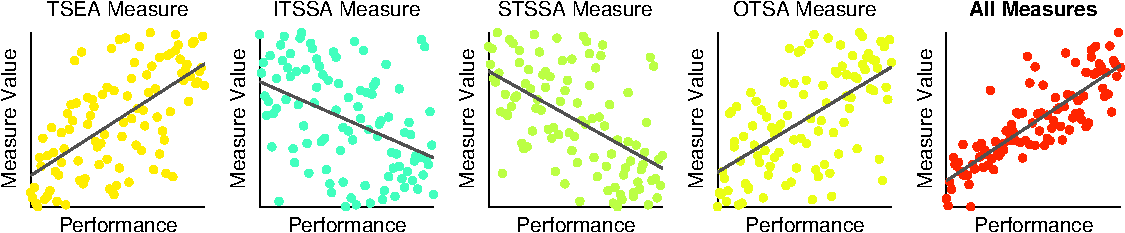
\includegraphics[width=\linewidth]{Figs/corr.pdf} \vspace{-1.0ex}
{\tiny \begin{spacing}{1.2} \textsf{\emph{TSEA: Task-related Stimulus Encoding Accuracy, ITSSA: Invariance \vs Task-related Stimulus Subspace Alignment, STSSA: Selectivity \vs Task-related Stimulus Subspace Alignment, OTSA: Optimal \vs Task-related Stimulus Alignment.}} \end{spacing}} \vspace{-0.5ex}
\end{minipage} %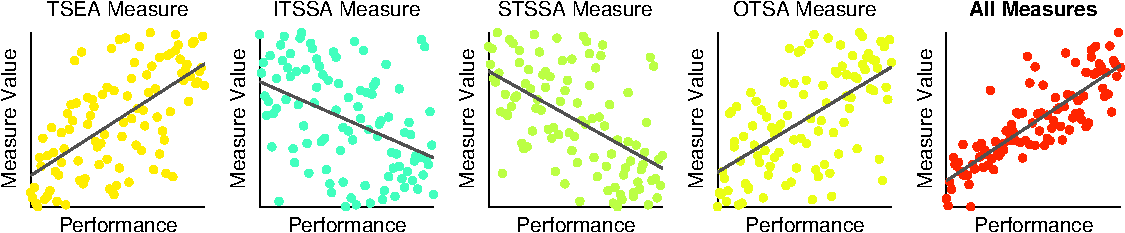
\includegraphics[width=0.90\textwidth]{Figs/corr.pdf}
\caption{{\bf Representation measures \vs performance of networks.}
Spearman's rank correlations ($\rho$) and their significance levels\protect\footref{fnote:defstars}~of the 4 measures and all measures\protect\footnotemark~together (using linear multiple correlation analysis) against the network's performance are $0.64^{\ast\ast\ast}$, $-0.44^{\ast\ast\ast}$, $-0.56^{\ast\ast\ast}$, $0.60^{\ast\ast\ast}$, and $0.84^{\ast\ast\ast}$, respectively (see supplementary material for full analysis). In other words, \emph{71\% of the variance ($\rho^2$) of deep networks' performances can be explained} using the proposed representation measures altogether.
}
\label{fig:corr}
\end{figure}

\footnotetext{The remainder of the measures that are included in the multiple correlation analysis but not individually reintroduced and shown in Fig.~\ref{fig:corr} are the invariance path potential, selectivity path potential, and invariance subspace capacity of vector representations. Their individual correlations and significance levels are $-0.31^{\ast\ast}$, $-0.24^{\ast}$, $-0.39^{\ast\ast\ast}$, respectively. See supplementary material for related details.}

{\bf Overall comparison.}
Spearman's rank correlations between all representation measures and all 100 deep networks' performances are summarized in Fig.~\ref{fig:corr}, and 71\% of the variance of deep networks' performances is explainable with the proposed measures altogether.
These measures further quantify the differences among deep representations and suggest features like network's 
encoding accuracies, invariance and selectivity subspaces' alignment, and optimal stimuli's alignment, against the task-related stimuli, can be extremely important for the effectiveness of deep representations.
Worth to note, although the first-order properties (TSEA and OTSA) do have stronger individual correlations, they cannot explain more about the network's performance than the other second-order properties ($0.56$ \vs $0.58$, again using linear multiple correlation analysis).

%Invariance and selectivity path potentials\footnote{\defvecpp} and invariance subspace capacity\footnote{\expinsc} for deep vector representations, on the contrary, have lower correlations to network's performance (though still significant), possibly due to their nature of being less task-related\footnote{\expextrinsic} than subspace alignment measures.

%Network's invariance subspace capacity (in terms of population representation), which though has an $R^2=0.15$ correlation as well, is in fact negatively correlated to network's performance, mainly due to the fact that poor performing network's invariance path search results are usually noisier (as depicted in Fig.~\ref{fig:align}D), and thus should be interpreted differently from the unit representation cases. on the other hand, are weaker in explaining networks' performances (with $R^2=0.10/0.06$), due to the fact that all deep networks have high but less ranked invariance and selectivity.

%Encoding specificity, as a single representation measure, can best explain the deep network's performance. Though bearing strong similarity to the invariance path search in terms of mathematical formulations, encoding specificity is in fact a radically different and complementary measure, since its numerical optimization is not constrained through distances to the reference stimulus (while distance constraints can induce \emph{a priori} similarities); thus, it can better function as an unconstrained global characterization of the ``encoding landscape'' (i.e.~multivariate tuning landscape of a population) and estimate if the (reconstructed) stimuli that a deep network is invariant to are ``selective'' (i.e.~visually similar to original stimuli). 

\section{Discussion}

%how to intrepret results
{\bf Contributions of this work.}
Comparatively, the characterization of representations in this work is designed to be general and unbiased such that both first- and second-order methods can be supported for single neurons or groups of neurons, without assuming any \emph{de facto} property in the solutions (\eg invariance to parametric deformations).
With the strong statistical significances of results obtained from the large-scale experiments on 100 shallow and 100 deep convolutional networks, in total 6,400 artificial neurons, we argue that our observations toward answering the differences between (shallow \vs deep) and among (deep) representations are highly conclusive, which can be summarized as:
\begin{itemize}[leftmargin=*] % Main Findings
%\setlength\itemsep{0.0ex}
\item Complexity of representations quantitatively increases along with network's depth.
\item Unlike deep representations, which are invariant and selective at the same time, shallow representations are only invariant, not selective, and their capacities of invariance are significantly lower than deep representations'.
\item Both first-order properties of deep representations (TSEA and OTSA) are extremely important to deep network's performance.
\item All second-order properties of deep representations (in particular, ITSSA and STSSA) together are as important as the first-order properties, if not significantly more.
\end{itemize}

{\bf Future work.}
In this work, we studied the simplest forms of convolutional networks--- random ``shallow'' (one-layer) networks and the simplest ``deep'' (two-layer) network.
However, it is obviously highly desirable to extend such investigations to deeper networks, and to networks that have been trained on large amounts of data.
Though the methods and measures proposed here are neutral to the depth of networks, numerical challenges (\eg evaluation and convergence speed, quality of solutions, \etc) would need to be addressed in very deep networks.

Beyond explaining what properties make a deep representation good, it would be valuable too to incorporate these findings into learning even better representations (which are almost solely driven by bigger datasets nowadays), \eg, via regularizing the representation measures.  
We believe that this could be useful in accelerating or improving representation learning, particularly when data are scarce and representations are not easily transferable.
Finally, even though a decently high fraction of the variance in deep network's performance has been explained, how to further increase this number, if there is an upper bound (\eg limits from dataset itself), \etc, need to be further investigated.

%Secondly, statistical tests were extensively deployed to support observations reported in this paper, especially in the context of real applications (\ie LFW-a face recognition), which might seem still far-fetched to be fully explainable by mathematical theories.
%Nonetheless, we envision that combining more theoretical analyses which, \eg, have been adopted in various topics in understanding deep representations \cite{delalleau2011shallow, montufar2014number}, with statistical simulations can further empower us in answering other important questions in deep networks \cite{bengio2013deep}.

%%application
% application: where training data is scarse; actively regularize representations
% not deep in this work, but adding another layer(level), what would happen
% not only optimal stimulus; modulate the landscape
% theory works gave some general answers, we want to answer, in real apps, why.
% still, to combine with theory

%\clearpage

{\small
\bibliographystyle{ieee}
\bibliography{ref}
}

\end{document}
